\documentclass[12pt]{article}

\bibliography{sbc-template}

\usepackage{graphicx}
\usepackage{indentfirst}
\usepackage[utf8]{inputenc}
\usepackage{listings}
\usepackage{sbc-template}
\usepackage{url}

\sloppy

\title{Relatório da Atividade Prática: DGEMM}
\author{Andrés Gonzalez Vilhena\\
        David Moreira Jacinto da Silva\\
        Lucas da Silva Inocencio}

\address{Escola Politécnica da Universidade Federal do Rio de Janeiro (UFRJ)\\
  Rio de Janeiro -- RJ -- Brasil
\email{agv1@poli.ufrj.br, davidmoreirajacinto.20222@poli.ufrj.br}
\email{lucas.inocencio@poli.ufrj.br}
}

\begin{document}

\maketitle

\begin{abstract}
    This document presents a comprehensive report on the optimization of the DGEMM operation. The investigation focuses on optimizing the DGEMM algorithm using various techniques, including vectorization, AVX instructions, loop unrolling, cache blocking, and parallelization with multiple threads. Python was used as the baseline for comparison, and the optimization was carried out using C and intrinsic functions. The results demonstrate significant performance improvements, achieving speedups of up to 4296.63 compared to the Python implementation. The study highlights the importance of leveraging hardware-specific features and optimization techniques to achieve efficient matrix multiplication on modern computing systems.
\end{abstract}

\section{Enunciado}

As operações com matrizes formam o núcleo dos códigos científicos que executam nos maiores supercomputadores do mundo, assim dado a relevância dos problemas estudados e os custos associados com a operação dessas grandes máquinas faz-se necessário que essas operações sejam executadas de maneira extremamente eficiente no hardware disponível. Em processadores de propósito geral essa eficiência somente é alcançada se o programador adaptar seus códigos aos recursos disponíveis na microarquitetura, reorganizando os padrões de acesso aos dados e fazendo uso de recursos especiais como instruções vetoriais.

Para essa tarefa um grupo de no máximo 3 alunos devem realizar uma investigação do código do DGEMM seguindo os passos indicados nas seções “Going Faster” do livro texto. O grupo deve realizar sua própria investigação de como as técnicas apresentadas melhoram o desempenho do DGEMM em suas plataformas. Cada grupo deve produzir um relatório descritivo a ser entregue no final do período (data especificada na página da disciplina), onde esse relatório deve conter uma explicação do problema DGEMM, além de uma seção para cada uma das otimizações feitas seguindo o que é apresentado em nossas aulas.

\newpage
\newpage

\section{Introdução}

O código-fonte está disponível em: \\
\url{https://github.com/lucas-inocencio/computer-architecture}

O problema de \textbf{D}ouble-\textbf{P}recision \textbf{Ge}neral \textbf{M}atrix \textbf{M}ultiply (DGEMM) é fundamental na área de Álgebra Linear, envolvendo o produto de matrizes de ponto flutuante de dupla precisão. Essa operação é amplamente utilizada em ciência da computação para resolver diversos problemas científicos. A multiplicação de matrizes é uma operação computacionalmente intensiva, especialmente para matrizes de grande porte, tornando a otimização do DGEMM essencial para alcançar alto desempenho em aplicações numéricas e científicas.

A forma geral do problema DGEMM pode ser expressa como:

\[ C = \alpha \cdot A \cdot B + \beta \cdot C \]

onde:

\begin{itemize}
    \item $A$, $B$ e $C$ são matrizes de dimensões adequadas (MxK, KxN e MxN, respectivamente).
    \item $\alpha$ e $\beta$ são valores escalares usados para a escala das matrizes $A \cdot B$ e $C$, respectivamente.
    \item O operador $\cdot$ representa a multiplicação de matriz.
\end{itemize}

Contudo, usaremos uma forma simplificada:

\[ C = A \cdot B \]

onde:

\begin{itemize}
    \item $A$, $B$ e $C$ são matrizes quadradas (NxN, NxN e NxN, respectivamente).
    \item O operador $\cdot$ representa a multiplicação matriz-matriz.
\end{itemize}


Especificação da máquina para os testes:

\begin{itemize}
    \item AMD Ryzen 5 3400G
    \item 8GB RAM (Dual Channel)
    \item Windows 11 Pro 22H2
    \item GCC 13.1
    \item Python 3.11
\end{itemize}

\newpage
\newpage

\section{Desenvolvimento}

\subsection{Matrix Multiply in Python}

Para demonstrar o poder das ideias usaremos o código abaixo como base de comparação para as otimizações.

Trecho de código original retirado do livro:

\begin{lstlisting}
    n = len(A)
    for i in range(n):
        for j in range(n):
            for k in range(n):
                C[i][j] += A[i][k] * B[k][j]
\end{lstlisting}

\begin{table}[h]
    \centering
    \label{tab:python}
    \begin{tabular}{cccc}
        \textbf{size} & \textbf{time} & \textbf{std} \\
        32 & 0.005648 & 0.002063 \\
        64 & 0.048004 & 0.006445 \\
        128 & 0.366891 & 0.025504 \\
        256 & 2.873940 & 0.025432 \\
        512 & 24.524437 & 0.295540 \\
        1024 & 221.705985 & 1.308298 \\
    \end{tabular}
    \caption{Python}
\end{table}

\begin{figure}[h]
    \centering
    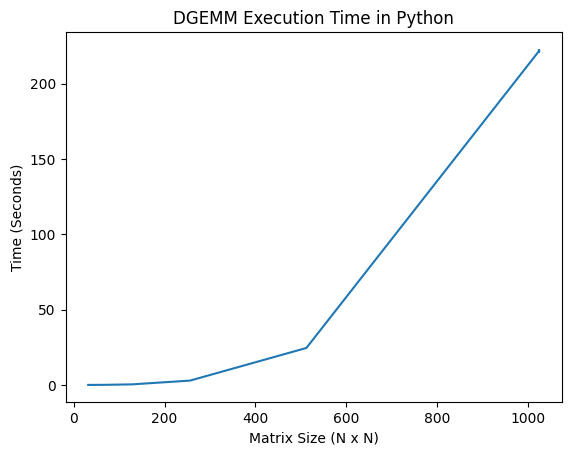
\includegraphics[scale=0.6]{figures/python.png}
    \caption{Python}
    \label{fig:python}
\end{figure}


Conforme mostrado na tabela de desempenho, mesmo para tamanhos de problemas relativamente pequenos, o Python exibe ineficiência na resolução de problemas de multiplicação de matrizes. Essa ineficiência se deve principalmente ao fato de o Python ser uma linguagem interpretada, o que normalmente resulta em uma execução mais lenta em comparação com as linguagens compiladas. Para tarefas computacionais intensas, como multiplicação de matrizes, é recomendável usar linguagens compiladas ou utilizar bibliotecas otimizadas para Python feitas em C ou Fortran, como NumPy ou Pandas, que podem melhorar significativamente o desempenho aproveitando otimizações e paralelização de baixo nível.

\newpage
\newpage

\subsection{Matrix Multiply in C}

Começamos reescrevendo o programa Python da subseção anterior. O código abaixo mostra uma versão de uma multiplicação matriz-matriz escrita em C. Como estamos passando a dimensão da matriz como parâmetro, esta versão do DGEMM usa versões unidimensionais de matrizes e aborda a aritmética para obter melhor desempenho, em vez de usar os arrays bidimensionais mais intuitivos que vimos no Python.

Trecho de código original retirado do livro:

\begin{lstlisting}
    for (int i = 0; i < n; ++i)
        for (int j = 0; j < n; ++j)
        {
            double cij = C[i + j * n];
            for (int k = 0; k < n; k++)
                cij += A[i + k * n] * B[k + j * n];
            C[i + j * n] = cij;
        }
\end{lstlisting}

\begin{table}[h]
    \centering
    \label{tab:gcc-flags}
    \begin{tabular}{cccc}
        \textbf{flag} & \textbf{time} & \textbf{std speedup} & \textbf{speedup} \\
        Python & 221.705985 & 0.0 & 1\\
        O0 &	 22.786200   &	0.308210  &	9.729836 \\
        O1 & 10.307400 & 0.280380 & 21.509400 \\
        O2 & 10.390800 & 0.264848 & 21.336758 \\
        O3 & 10.182000 & 0.385060 & 21.774306 \\
        Ofast & 11.214800 & 1.825751 & 19.769054 \\
    \end{tabular}
    \caption{gcc flags}
\end{table}

\begin{figure}[h]
    \centering
    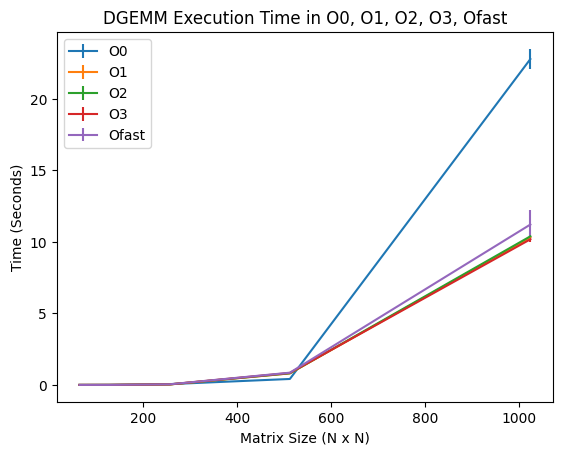
\includegraphics[scale=0.6]{figures/times_gcc.png}
    \caption{Times GCC Flags}
    \label{fig:times-gcc-flagsl}
\end{figure}

\begin{figure}[h]
    \centering
    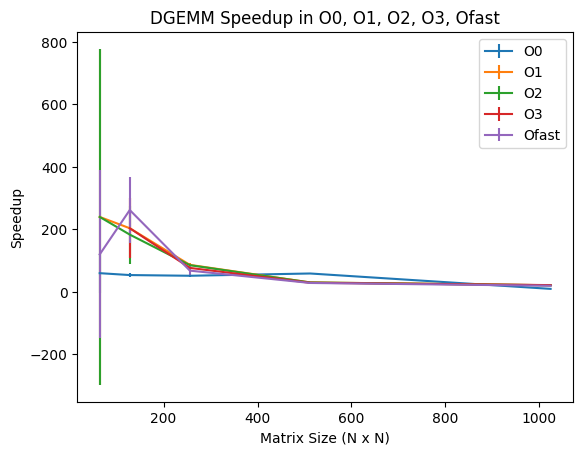
\includegraphics[scale=0.6]{figures/speedups_gcc.png}
    \caption{Speedups GCC Flags}
    \label{fig:speedups-gcc-flags}
\end{figure}

É evidente que usar uma linguagem compilada como C e aproveitar a localidade espacial (dado que C armazena matrizes contíguas na memória) pode melhorar significativamente o desempenho da multiplicação de matrizes. Além disso, o uso de sinalizadores de otimização gcc apropriados aumenta ainda mais a velocidade de execução, com o sinalizador O3 demonstrando o melhor desempenho entre os sinalizadores testados.

\newpage
\newpage

\subsection{Subword Parallelism and Matrix Multiply}

Para demonstrar o impacto no desempenho do paralelismo de subpalavras, executaremos novamente o código usando AVX. Embora os criadores de compiladores possam eventualmente produzir código de alta qualidade rotineiramente que usa as instruções AVX do x86, por enquanto iremos "trapacear" usando intrínsecos C que mais ou menos dizem ao compilador exatamente como produzir um bom código. 

A declaração na linha 7 da Figura 3.19 usa o tipo de dados m256d, que informa o compilador a variável conterá quatro valores de ponto flutuante de precisão dupla (4 x 64 bits = 512 bits).

O intrínseco mm256loadpd(), também na linha 7, usa instruções AVX para carregar quatro números de ponto flutuante de precisão dupla em paralelo (pd) da matriz C para c0. O cálculo do endereço C+i+j*n representa o elemento C[i+j*n]. Simetricamente, a etapa final na linha 13 usa o mm256storepd() intrínseco para armazenar oito números de ponto flutuante de precisão dupla de c0 na matriz C. À medida que passamos por oito elementos a cada iteração, o loop for externo na linha 4 incrementa i em 8 em vez de 1 como na linha 3 da Figura 2.43 do Capítulo 2.

Dentro dos loops, na linha 10 primeiro carregamos quatro elementos de A novamente usando mm256loadpd(). Para multiplicar esses elementos por um elemento de B, primeiro usamos o intrínseco mm256broadcastsd(), que faz quatro cópias idênticas do número escalar de dupla precisão - neste caso, um elemento de B - em um dos registradores ZMM. Em seguida, usamos mm256fmaddpd na linha 11 para multiplicar os quatro resultados de precisão dupla em paralelo e, em seguida, adicionar os quatro produtos às quatro somas em c0.

Trecho de código original retirado do livro:

\begin{lstlisting}
    for (int i = 0; i < n; i += 4)
        for (int j = 0; j < n; j++)
        {
            __m256d c0 = _mm256_load_pd(C + i + j * n);
            for (int k = 0; k < n; k++)
                c0 = _mm256_add_pd(c0,
                     _mm256_mul_pd(_mm256_load_pd(A+i+k*n),
                     _mm256_set1_pd(B[k + j * n])));
            _mm256_store_pd(C + i + j * n, c0);
        }
    for (int i = 0; i < n; i += 4)
        for (int j = 0; j < n; j++)
        {
            __m256d c0 = _mm256_load_pd(C + i + j * n);
            for (int k = 0; k < n; k++)
                c0 = _mm256_add_pd(c0,
                     _mm256_mul_pd(_mm256_load_pd(A+i+k*n),
                     _mm256_broadcast_sd(B + k + j * n)));
            _mm256_store_pd(C + i + j * n, c0);
        }
\end{lstlisting}

\begin{table}[h]
    \centering
    \label{tab:avx}
    \begin{tabular}{cccc}
        \textbf{Type} & \textbf{time} & \textbf{std speedup} & \textbf{speedup} \\
        None & 148.329424 & 1.825751 & 19.769054 \\
        AVX &	20.996636	 &	1.838429 &	137.563176\\
        AVX2 &	21.419500	 &	3.335001 &	138.375974\\
    \end{tabular}
    \caption{AVX}
\end{table}

\begin{figure}[h]
    \centering
    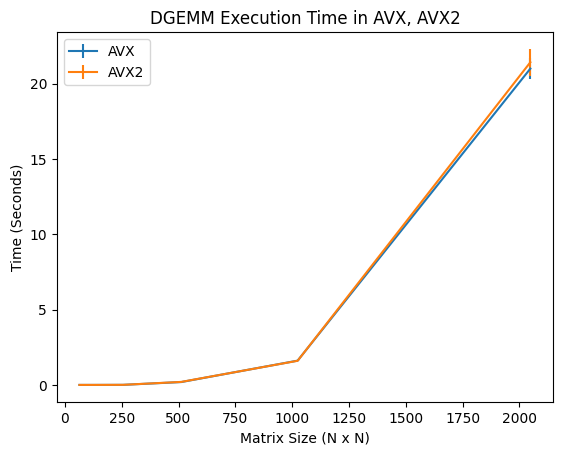
\includegraphics[scale=0.6]{figures/times_avx.png}
    \caption{Times AVX Instructions}
    \label{fig:times-avx}
\end{figure}

\begin{figure}[h]
    \centering
    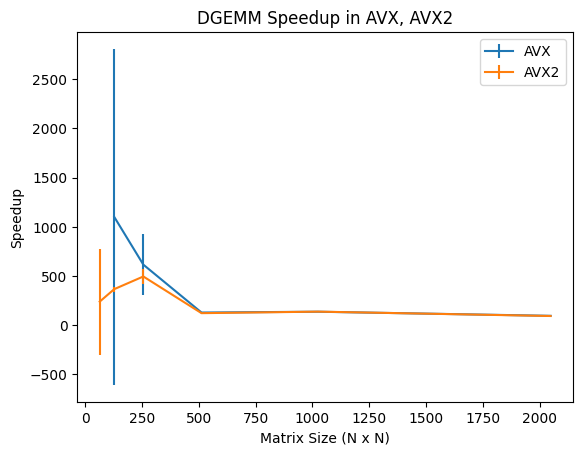
\includegraphics[scale=0.6]{figures/speedups_avx.png}
    \caption{Speedups AVX Instructions}
    \label{fig:speedups-avx}
\end{figure}

A versão AVX2 é 7.0 vezes mais rápida, o que é muito próximo do fator de aumento de 8,0 que você pode esperar ao executar oito vezes mais operações por vez usando o paralelismo de subpalavras.

\newpage
\newpage

\subsection{Instruction-Level Parallelism and Matrix Multiply}

Nesta seção, discutiremos o código apresentado, que explora o paralelismo de nível de instrução (Instruction-Level Parallelism - ILP). Podemos ver o impacto do paralelismo em nível de instrução ao desenrolar o loop de modo que o processador de execução fora de ordem e com vários problemas tenha mais instruções para trabalhar. Como o exemplo de desenrolamento no código abaixo, vamos desenrolar o loop quatro vezes. Em vez de desenrolar manualmente o loop em C fazendo quatro cópias de cada um dos intrínsecos na , podemos contar com o compilador gcc para fazer o desenrolar na otimização -O3. (Usamos a constante UNROLL no código C para controlar a quantidade de desenrolamento caso desejemos tentar outros valores.) Cercamos cada intrínseco com um loop for simples com quatro iterações (linhas 9, 15 e 19) e substituímos o escalar C0 por um array de quatro elementos c[] (linhas 8, 10, 16 e 20).

Trecho de código original retirado do livro:

\begin{lstlisting}
    for (int i = 0; i < n; i += UNROLL * 4)
        for (int j = 0; j < n; ++j)
        {
            __m256d c[UNROLL];
            for (int r = 0; r < UNROLL; r++)
                c[r] = _mm256_load_pd(C + i + r * 4 + j * n);
    
            for (int k = 0; k < n; k++)
            {
                __m256d bb = _mm256_broadcast_sd(B + j * n + k);
                for (int r = 0; r < UNROLL; r++)
                    c[r] = _mm256_fmadd_pd(_mm256_load_pd(A+n*k+r*4+i), 
                                          bb, c[r]);
            }
            for (int r = 0; r < UNROLL; r++)
                _mm256_store_pd(C + i + r * 4 + j * n, c[r]);
        }
\end{lstlisting}

\begin{table}[h]
    \centering
    \label{tab:unroll}
    \begin{tabular}{cccc}
        \textbf{Num\_UNROLL} & \textbf{time} & \textbf{std speedup} & \textbf{speedup} \\
        1 & 21.419500 & 3.335001 & 138.375974 \\
        2 & 14.011400 & 3.475817 & 144.415050 \\
        4 & 11.466800 & 3.036342 & 198.270421 \\
        8 & 9.664400 & 3.251052 & 288.754864 \\
        16 & 8.587600 & 7.057091 & 325.082089 \\
        32 & 9.390600 & 2.875658 & 199.160964 \\
    \end{tabular}
    \caption{UNROLL}
\end{table}

\begin{figure}[h]
    \centering
    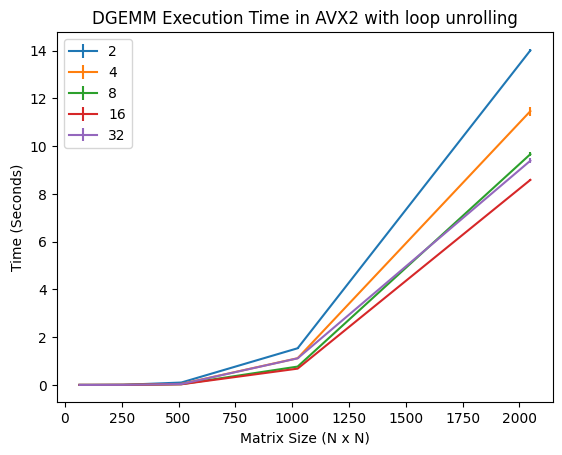
\includegraphics[scale=0.6]{figures/times_unroll.png}
    \caption{Times UNROLL}
    \label{fig:times-unroll}
\end{figure}

\begin{figure}[h]
    \centering
    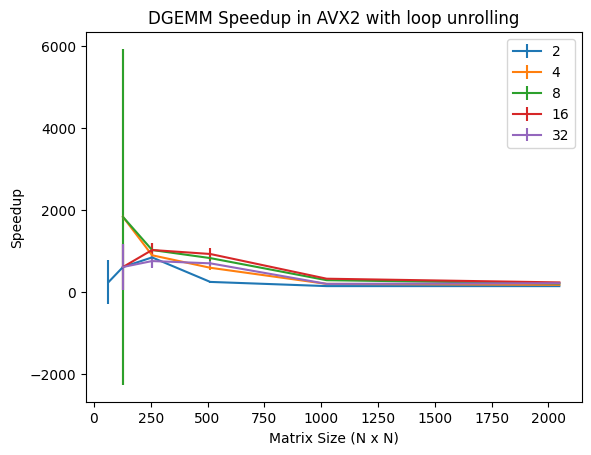
\includegraphics[scale=0.6]{figures/speedups_unroll.png}
    \caption{Speedups UNROLL}
    \label{fig:speedups-unroll}
\end{figure}

As otimizações para paralelismo de subpalavra e paralelismo em nível de instrução resultam em um aumento geral de velocidade de 2.35 em relação ao DGEMM anterior. Comparado com a versão do Python é 325 vezes mais rápido.

\newpage
\newpage

\subsection{Cache Blocking and Matrix Multiply}

O blocking de cache é uma técnica usada para melhorar o desempenho dos algoritmos array-like, aproveitando a hierarquia de memória. O objetivo é dividir a matriz de multiplicação em blocos menores que caibam no cache, reduzindo cache miss e melhorando a localidade dos dados. O código abaixo a versão blocking. O benefício do bloqueio aumenta com o tamanho da matriz. Como o número de operações de ponto flutuante por elemento de matriz é o mesmo independente do tamanho da matriz, podemos medir o desempenho de maneira justa pelo número de operações de ponto flutuante computadas por segundo. A Figura 5.49 compara o desempenho em GFLOPS/seg da versão C original com

Trecho de código original retirado do livro:

\begin{lstlisting}
    void do_block(int n, int si, int sj, int sk, double *A, 
                double *B, double *C)
    {
        for (int i = si; i < si + BLOCKSIZE; ++i)
            for (int j = sj; j < sj + BLOCKSIZE; ++j)
            {
                double cij = C[i + j * n];
                for (int k = sk; k < sk + BLOCKSIZE; k++)
                    cij += A[i + k * n] * B[k + j * n];
                C[i + j * n] = cij;
            }
    }

    for (int sj = 0; sj < n; sj += BLOCKSIZE)
        for (int si = 0; si < n; si += BLOCKSIZE)
            for (int sk = 0; sk < n; sk += BLOCKSIZE)
                do_block(n, si, sj, sk, A, B, C);
\end{lstlisting}

\begin{table}[h]
    \centering
    \label{tab:blocking}
    \begin{tabular}{cccc}
        \textbf{blocksize} & \textbf{time} & \textbf{std speedup} & \textbf{speedup} \\
        2 & 2741.971699 & 0.753559	& 6.945720 \\
        4 & 532.456043 & 0.377248	&29.855371 \\
        8 & 171.177093	 & 0.851576	&90.967497 \\
        16 & 62.3320 & 5.452846	&237.728914 \\
        32 & 36.7116 & 41.334782	&558.172167 \\
        64 & 18.9454 & 106.366971&	1171.807531\\
        128 & 10.3458 & 180.797594&	1805.423330\\
        256 & 36.8776 & 285.966855&	1613.580676\\
    \end{tabular}
    \caption{Blocking}
\end{table}

\begin{figure}[h]
    \centering
    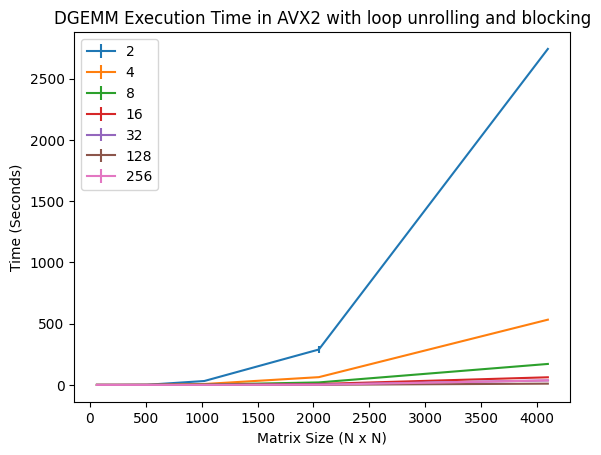
\includegraphics[scale=0.6]{figures/times_blocking.png}
    \caption{Times Blocking}
    \label{fig:times-blocking}
\end{figure}

\begin{figure}[h]
    \centering
    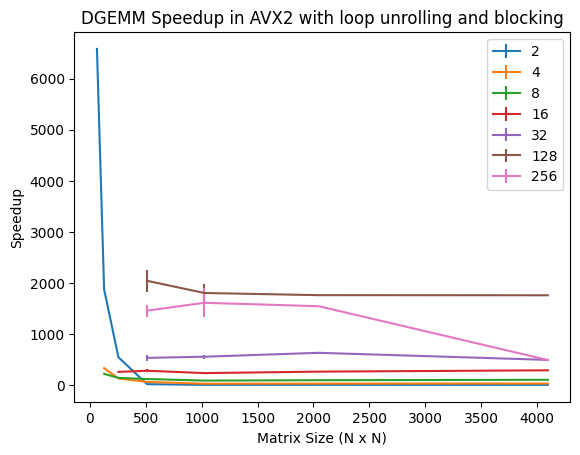
\includegraphics[scale=0.6]{figures/speedups_blocking.png}
    \caption{Speedups Blocking}
    \label{fig:speedups-blocking}
\end{figure}

Otimizações para paralelismo de subpalavra, paralelismo em nível de instrução e caches. O caching melhora o desempenho sobre o código anterior por fatores 56 para a maior matriz. A menor matriz cabe no cache L1, então o cache quase não faz diferença.

\newpage
\newpage

\subsection{Multiple Processors and Matrix Multiply}

Esta seção é a final. Cada Core Ryzen 5 3400G tem quatro núcleos e oito threads. O código abaixo mostra a versão OpenMP do DGEMM que utiliza esses núcleos. Observe que a linha 27 é a única linha adicionada para fazer esse código rodar em vários processadores: um pragma OpenMP que informa ao compilador para usar vários threads no loop mais externo. Ele diz ao computador para espalhar o trabalho do loop mais externo por todos os threads. A Figura traça um gráfico clássico de aceleração de multiprocessador, mostrando a melhoria de desempenho em relação a um único thread à medida que o número de threads aumenta. Este gráfico facilita a visualização dos desafios de strong scaling versus weak scaling. Quando tudo cabe no cache de dados de primeiro nível, como é o caso de matrizes 64 × 64, adicionar threads na verdade prejudica o desempenho. A versão de 48 threads do DGEMM é quase metade da velocidade da versão de thread único neste caso. Em contraste, as duas maiores matrizes obtêm uma aceleração de 8 e, portanto, as clássicas duas linhas “para cima e para a direita”.Na versão Python, a aceleração é de quase 5.000 para uma versão C do DGEMM otimizada para paralelismo de nível de dados, hierarquia de memória e paralelismo de nível de thread.

Trecho de código original retirado do livro:

\begin{lstlisting}
    void do_block(int n, int si, int sj, int sk,
                   double *A, double *B, double *C)
    {
        for (int i = si; i < si + BLOCKSIZE; i += UNROLL * 4)
            for (int j = sj; j < sj + BLOCKSIZE; j++)
            {
                __m256d c[UNROLL];
                for (int r = 0; r < UNROLL; r++)
                    c[r] = _mm256_load_pd(C + i + r * 4 + j * n);
                for (int k = sk; k < sk + BLOCKSIZE; k++)
                {
                    __m256d bb = _mm256_broadcast_sd(B + j * n + k);
                    for (int r = 0; r < UNROLL; r++)
                        c[r]=_mm256_fmadd_pd(_mm256_load_pd(A+n*k+r*4+i)
                                            , bb, c[r]);
                }
    
                for (int r = 0; r < UNROLL; r++)
                    _mm256_store_pd(C + i + r * 4 + j * n, c[r]);
            }
    }
\end{lstlisting}

\begin{lstlisting}
    omp_set_num_threads(P);
    #pragma omp parallel for
        for (int sj = 0; sj < n; sj += BLOCKSIZE)
            for (int si = 0; si < n; si += BLOCKSIZE)
                for (int sk = 0; sk < n; sk += BLOCKSIZE)
                    do_block(n, si, sj, sk, A, B, C);
\end{lstlisting}

\begin{table}[h]
    \centering
    \label{tab:threads}
    \begin{tabular}{cccc}
        \textbf{threads} & \textbf{time} & \textbf{std speedup} & \textbf{speedup} \\
        1 & 319.6388 & 180.797594 & 1805.423330 \\
        2 & 118.9168 & 461.010250	& 2849.691322 \\
        4 & 65.4736 & 969.264761	& 4638.200520 \\
        8 & 49.1352	 & 	361.930530	& 4296.627614 \\
    \end{tabular}
    \caption{Threads}
\end{table}

\begin{figure}[h]
    \centering
    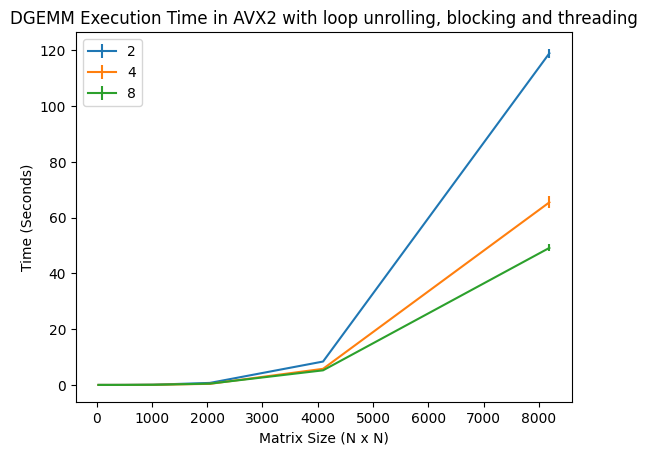
\includegraphics[scale=0.6]{figures/times_threads.png}
    \caption{Times Threads}
    \label{fig:times-threads}
\end{figure}

\begin{figure}[h]
    \centering
    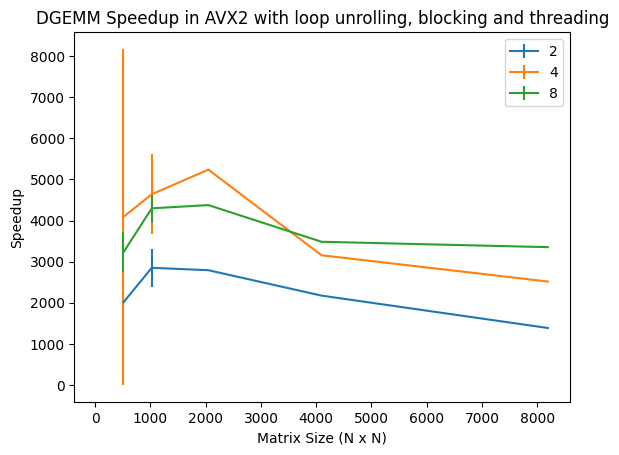
\includegraphics[scale=0.6]{figures/speedups_threads.png}
    \caption{Speedups Threads}
    \label{fig:speedups-threads}
\end{figure}

A utilização de múltiplos processadores (ou threads) para realizar a multiplicação de matrizes em paralelo, usando a biblioteca OpenMP, demonstra um grande aumento no desempenho em relação à execução sequencial. O uso de 8 threads alcançou uma velocidade quase 6.5 vezes maior em comparação com o desempenho sequencial.

\newpage
\newpage

\section{Resultados}

\begin{table}[h]
    \centering
    \label{tab:final}
    \begin{tabular}{cccc}
        \textbf{Chapter} & \textbf{time} & \textbf{std speedup} & \textbf{speedup} \\
        1 & 164691.596770 & 0.0 & 1 \\
        2 & 25472.162249	 & 1.825751 &	19.769054 \\
        3 & 8877.037799 & 3.335001 &	138.375974 \\
        4 & 666.024234	 & 	7.057091	& 325.082089 \\
        5 & 319.6388	 & 	180.797594 &	1805.423330 \\
        6 & 49.1352	 & 	361.930530	& 4296.627614 \\
    \end{tabular}
    \caption{Comparação Final}
\end{table}

\begin{figure}[h]
    \centering
    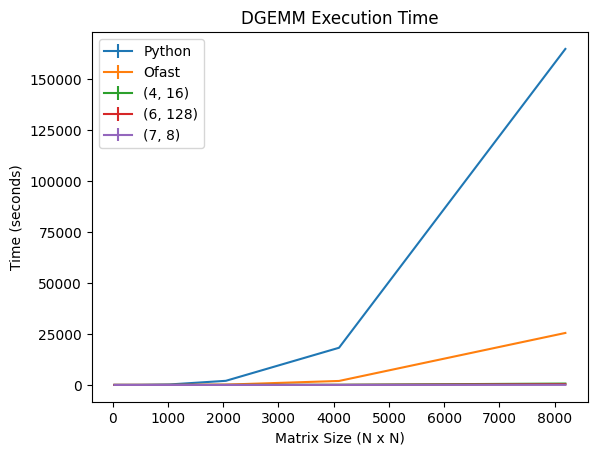
\includegraphics[scale=0.6]{figures/all_times_sizes.png}
    \caption{Comparação Final Tempos}
    \label{fig:times-finall}
\end{figure}

\begin{figure}[h]
    \centering
    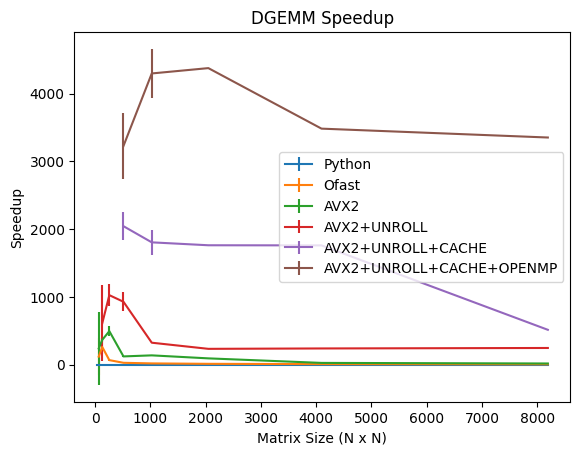
\includegraphics[scale=0.6]{figures/all_speedups_sizes.png}
    \caption{Comparação Final Speedups}
    \label{fig:speedups-final}
\end{figure}

\newpage
\newpage

\section{Referências}

\begin{enumerate}
\item \textit{Computer Organization and Design RISC-V Edition: The Hardware Software Interface}, 2nd edition, by David A. Patterson and John L. Hennessy. Morgan Kaufmann, 2021.

\item \textit{Computer Organization and Architecture: Designing for Performance}, 11th edition, by William Stallings. Pearson, 2022.

\item \textit{Digital Design Using VHDL: A Systems Approach} by John F. Wakerly. Pearson, 2016.

\item Especificações AMD Ryzen 5 3400G retirado de \url{https://en.wikichip.org/wiki/amd/ryzen_5/3400g}

\item Microarquitetura Zen+ retirado de \url{https://en.wikichip.org/wiki/amd/microarchitectures/zen}

\item Documentação GCC retirado de \url{https://gcc.gnu.org/onlinedocs/gcc}

\end{enumerate}

\end{document}